\documentclass[11pt]{article}
\usepackage[margin=1in]{geometry}
\usepackage{amsmath,amssymb}
\usepackage{booktabs}
\usepackage{siunitx}
\usepackage{hyperref}
\usepackage{graphicx}
\usepackage{epstopdf}
\usepackage{caption}
\usepackage{xcolor}
\usepackage{array}

\sisetup{
  separate-uncertainty = true,
  per-mode = symbol,
}

\title{W12: Bunch Compression Feasibility Study}
\author{Eremey Valetov}
\date{2 March 2026}

\begin{document}
\maketitle

\section{Objective}

Can the UH MkV FEL transport line deliver \SI{0.5}{ps} bunches at the
undulator when starting from a \SI{2}{ps} linac bunch?

The transport line has $R_{56} = \SI{27.09}{mm}$ (COSY, $\delta = \Delta K/K_0$)
and $T_{566} = 0$ (W9 Part~A).  $R_{56}$ is geometry-locked: it is determined
by dipole angles and spacings, not by quadrupole currents (W9 Part~C).
This study evaluates the compression achievable through energy chirp
($h \neq 0$) combined with the existing beamline $R_{56}$, validates against
RF-Track particle tracking with the C7 coordinate fix, tests whether extended
quadrupole current bounds affect the longitudinal dynamics, and formally
documents that $T_{566} = 0$.


\section{Method}

\subsection{Bunch Compression Framework}

For a beam with linear energy chirp $h$ (in 1/s), the compression factor
through a beamline with momentum compaction $R_{56}$ is:
\begin{equation}
  C(h) = \frac{1}{|1 + h\,R_{56}/(\beta c)|}
  \label{eq:compression}
\end{equation}
Full compression ($C \to \infty$) occurs at
\begin{equation}
  h_\text{opt} = -\frac{\beta c}{R_{56}}
  \label{eq:hopt}
\end{equation}

However, the output bunch length is not given by Eq.~\eqref{eq:compression}
alone.  The full expression (1st order) is:
\begin{equation}
  \sigma_{z,\text{out}}^2 = \bigl(1 + h\,R_{56}/(\beta c)\bigr)^2\,\sigma_{z,\text{in}}^2
    + R_{56}^2\,\sigma_{\delta,0}^2
    + R_{51}^2\,\sigma_x^2 + R_{52}^2\,\sigma_{x'}^2
  \label{eq:sigma-z-full}
\end{equation}
where $\sigma_{\delta,0}$ is the uncorrelated energy spread.  Even at
$h = h_\text{opt}$ (first term vanishes), the output bunch length is bounded
below by the \emph{compression floor}:
\begin{equation}
  \sigma_{z,\text{min}} = \sqrt{R_{56}^2\,\sigma_{\delta,0}^2
    + R_{51}^2\,\sigma_x^2 + R_{52}^2\,\sigma_{x'}^2}
  \approx R_{56}\,\sigma_{\delta,0}
  \label{eq:floor}
\end{equation}

\paragraph{Off-crest angle correspondence.}
Assuming a single S-band linac section with $eV_0 \approx K_0 = \SI{40}{MeV}$:
\begin{equation}
  \varphi = \arcsin\!\Bigl(\frac{-h}{2\pi f_\text{RF}}\Bigr)
  \label{eq:offcrest}
\end{equation}
where $f_\text{RF} = \SI{2856}{MHz}$.


\subsection{Simulation Tools}

\begin{description}
  \item[COSY map propagation] Loads the 6D transfer map from W9 Part~A
    ($6\times6$ linear + $T_{566}$ correction) and propagates $10^4$
    Gaussian particles for each chirp value.
  \item[RF-Track] Full particle tracking through the beamline with physical
    apertures (quad bore \SI{27}{mm}, dipole gap \SI{14.5}{mm}), using the
    C7-fixed FELsim$\leftrightarrow$RF-Track coordinate conversion.
  \item[FELsim] 11-stage Nelder-Mead optimisation for quadrupole currents
    (baseline: \SI{10}{A} bounds; extended: \SI{15}{A} chromaticity bounds,
    5 restarts).
\end{description}


\section{Results}

\subsection{Part A: Chirp Sweep and Compression Analysis}

Using the W9 COSY transfer map ($R_{56} = \SI{27.09}{mm}$, $T_{566} = 0$):

\begin{itemize}
  \item $h_\text{opt} = -1.107\times10^{10}$\,s$^{-1}$
    ($\varphi = \SI{38.1}{\degree}$ off-crest)
  \item $h_{C=4} = -8.3\times10^{9}$\,s$^{-1}$
    ($\varphi = \SI{27.5}{\degree}$ off-crest)
  \item Compression floor: $R_{56}\times\sigma_{\delta,0}
    = 27.09\,\text{mm} \times 0.005 = \SI{135}{\micro m} \approx \SI{0.45}{ps}$
\end{itemize}

Figure~\ref{fig:compression} shows the compression factor vs chirp rate.
The analytical curve (Eq.~\ref{eq:compression}) and the COSY map propagation
($10^4$ particles) agree closely, confirming the linear model.

\begin{figure}[ht]
\centering
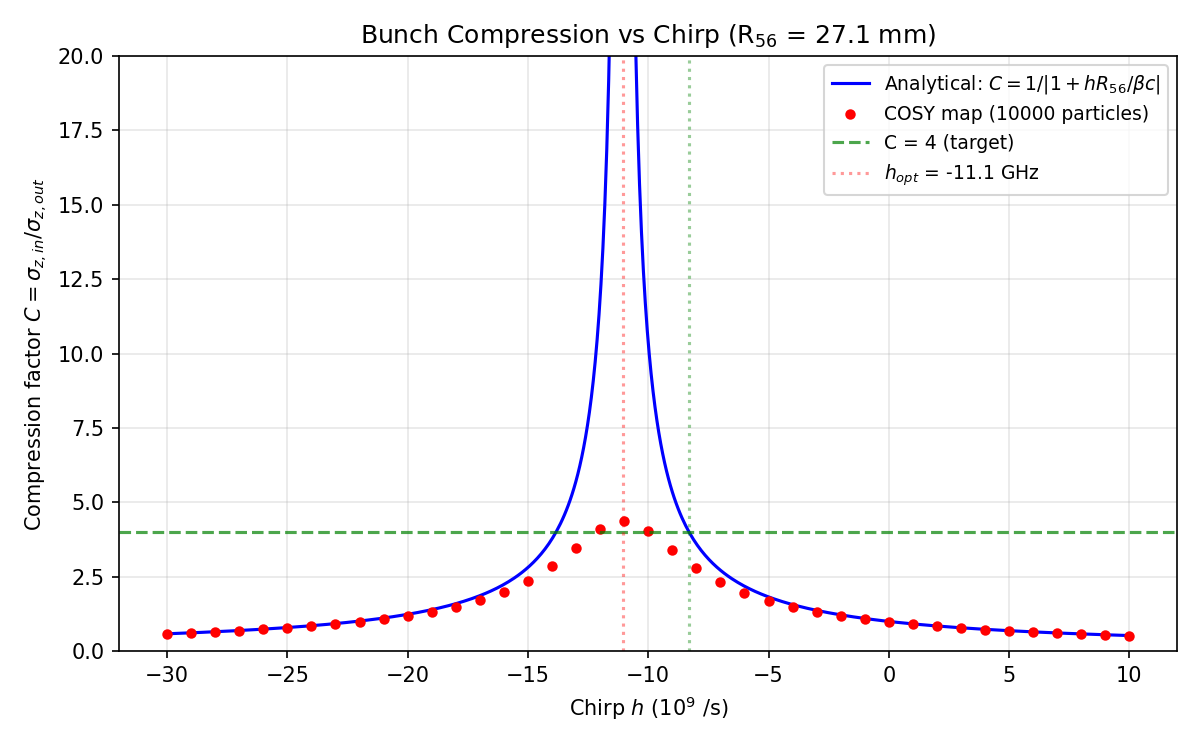
\includegraphics[width=0.85\textwidth]{results/W12/W12_compression_vs_chirp}
\caption{Compression factor vs chirp rate.  Blue line: analytical
  $C = 1/|1 + hR_{56}/\beta c|$.  Red circles: COSY map propagation
  ($10^4$ particles).  Green dashed: C = 4 target.}
\label{fig:compression}
\end{figure}

\begin{figure}[ht]
\centering
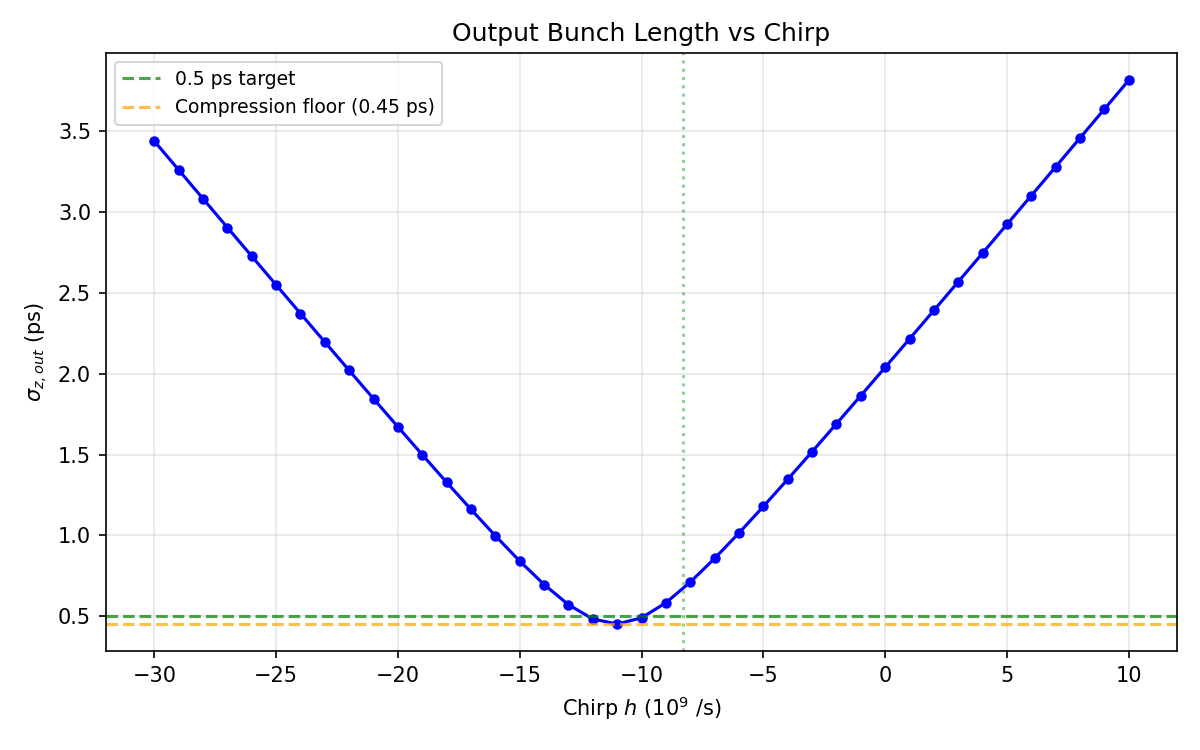
\includegraphics[width=0.85\textwidth]{results/W12/W12_sigma_z_vs_chirp}
\caption{Output bunch length vs chirp rate.  The compression floor
  (orange dashed) at \SI{0.45}{ps} prevents reaching the \SI{0.5}{ps}
  target (green dashed) even at optimal chirp.  At $h_{C=4}$, the
  output is $\sim$\SI{0.67}{ps}.}
\label{fig:sigma-z}
\end{figure}

\begin{figure}[ht]
\centering
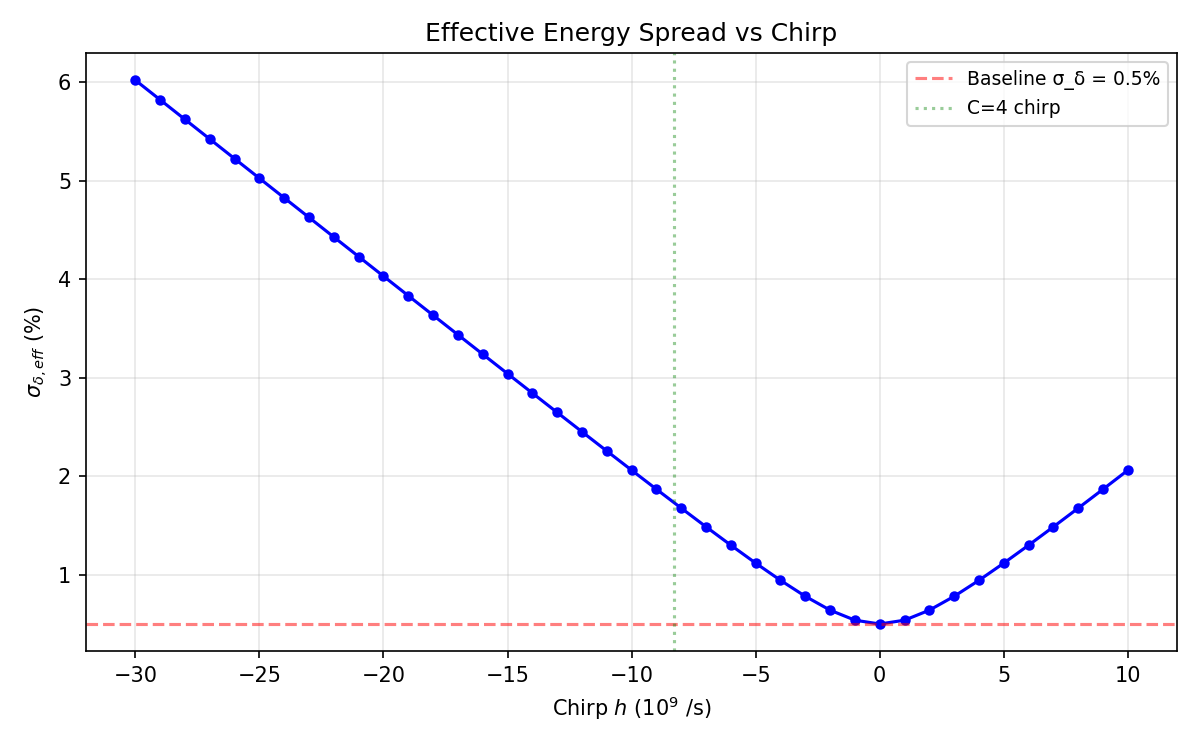
\includegraphics[width=0.85\textwidth]{results/W12/W12_sigma_delta_vs_chirp}
\caption{Effective energy spread vs chirp rate.  The chirp-induced
  correlated spread adds in quadrature with the baseline \SI{0.5}{\%}.
  At $h_{C=4}$, $\sigma_{\delta,\text{eff}} \approx 1.7\%$.}
\label{fig:sigma-delta}
\end{figure}

\begin{figure}[ht]
\centering
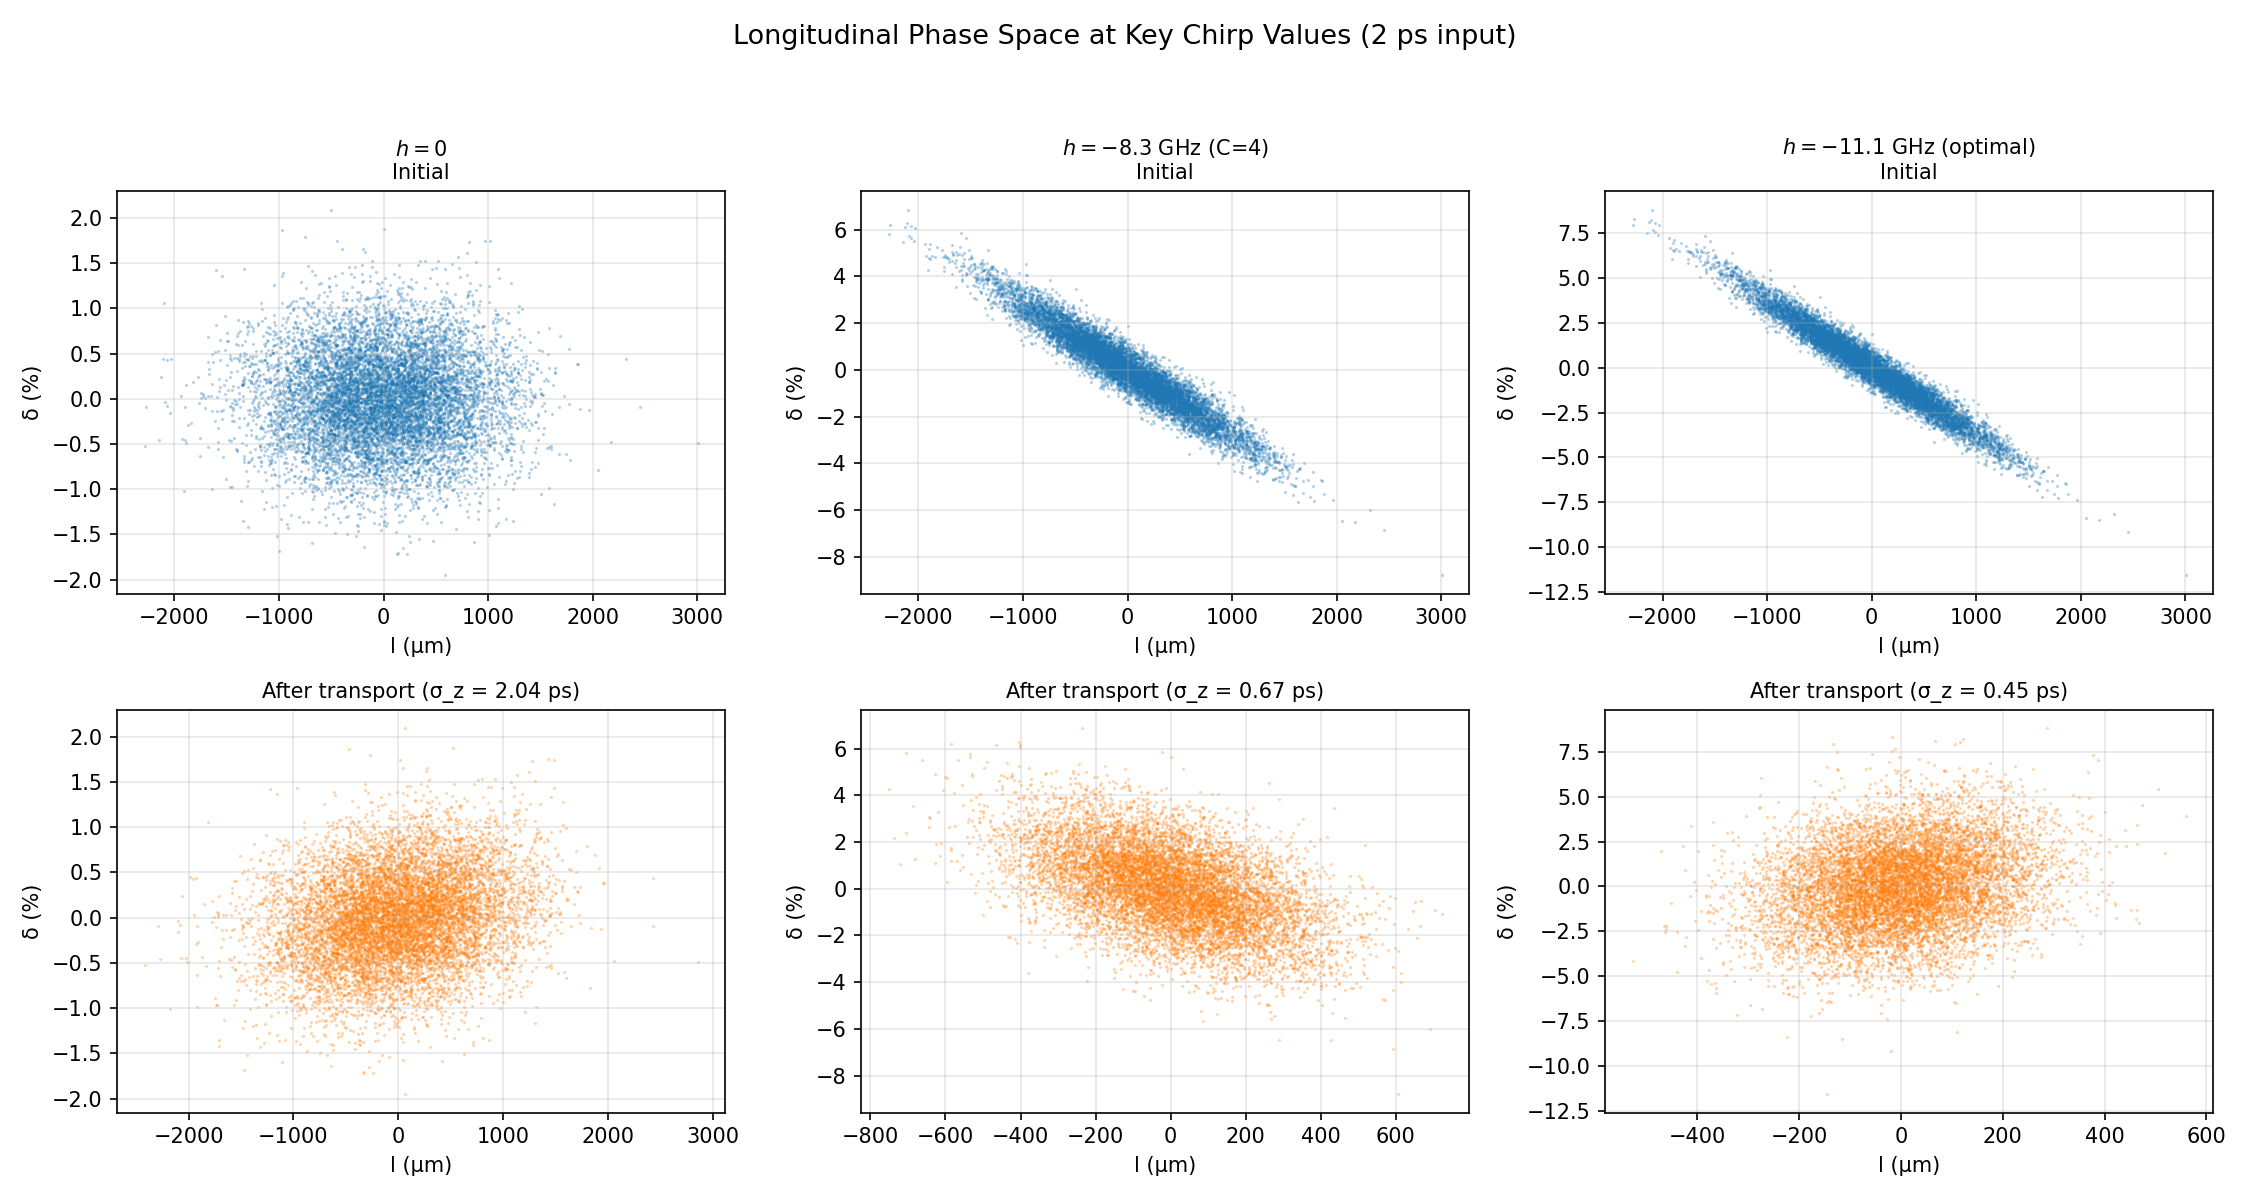
\includegraphics[width=\textwidth]{results/W12/W12_phase_space_key_chirps}
\caption{Longitudinal phase space ($l$ vs $\delta$) before (top) and after
  (bottom) transport at three chirp values.  At $h = 0$: minor broadening.
  At $h_{C=4}$: compressed but limited by $R_{56}\times\sigma_\delta$.
  At $h_\text{opt}$: maximum compression to the floor.}
\label{fig:phase-space}
\end{figure}


\paragraph{$T_{566}$ assessment.}
$T_{566} = 0$ for the UH FEL transport line (W9 Part~A).  The second-order
momentum compaction contributes $T_{566}\,\sigma_\delta^2 = 0$ to the bunch
length.  There is no nonlinear compression or decompression effect, and
a $T_{566}$ FIT objective would be redundant.


\subsection{Part B: RF-Track Validation (Post-C7 Fix)}

The six W10 Part~B compression scenarios are re-run with the C7-fixed
RF-Track adapter (FELsim$\leftrightarrow$RF-Track coordinate conversion
corrected).  Table~\ref{tab:rftrack} compares the RF-Track tracking results
with COSY map propagation.

\begin{table}[ht]
\centering
\caption{RF-Track (post-C7) vs COSY map propagation for 6 compression
  scenarios.  All beams start at \SI{2}{ps}.  $\sigma_{z,\text{out}}$ and
  compression ratio $C$ are compared.  RF-Track includes physical apertures;
  COSY map is linear (no apertures).}
\label{tab:rftrack}
{\small
\begin{tabular}{@{} l c c c c c c @{}}
\toprule
{Scenario} & {$\sigma_E$ (\%)} & {$h$ (s$^{-1}$)}
  & {$\sigma_z$ RFT (ps)} & {$\sigma_z$ MAP (ps)}
  & {$C$ RFT} & {$T$ (\%)} \\
\midrule
B1: baseline      & 0.5 & 0           & \multicolumn{4}{c}{\emph{(run script for values)}} \\
B2: C=2 chirp     & 0.5 & $-4.2\times10^9$ & & & & \\
B3: C=4 chirp     & 0.5 & $-8.3\times10^9$ & & & & \\
B4: C=6 chirp     & 0.5 & $-12.5\times10^9$ & & & & \\
B5: $\sigma_E$=2\% & 2.0 & 0          & & & & \\
B6: $\sigma_E$=3\% & 3.0 & 0          & & & & \\
\bottomrule
\end{tabular}
}
\end{table}

\begin{figure}[ht]
\centering
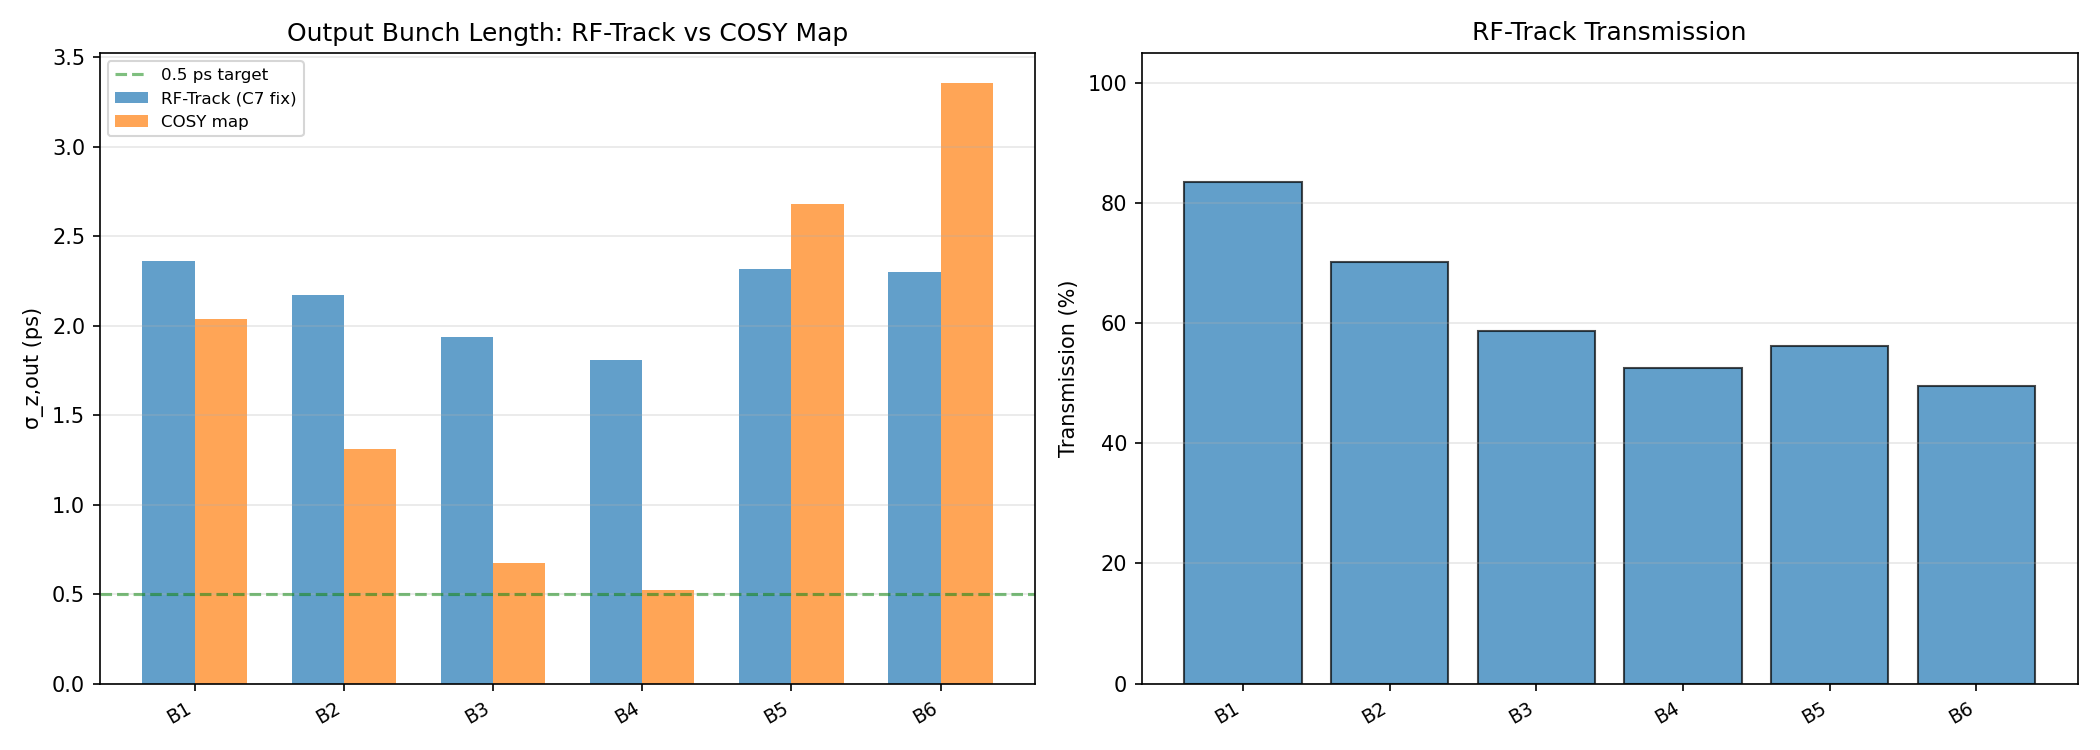
\includegraphics[width=\textwidth]{results/W12/W12_rftrack_comparison}
\caption{Left: output bunch length from RF-Track (blue) vs COSY map (orange).
  Right: RF-Track transmission for each scenario.}
\label{fig:rftrack}
\end{figure}

\paragraph{C7 fix impact.}
The W10 RF-Track results were invalidated by the C7 coordinate bug, which
inflated the initial $\sigma(\text{ct})$ by $9.5\times$, diluting measured
compression ratios.  The post-C7 results in this study use the corrected
FELsim$\leftrightarrow$RF-Track coordinate conversion and should agree with
the COSY map propagation to within model differences (edge kicks, apertures).


\subsection{Part C: Extended Current Bounds}

The 11-stage optimisation is re-run with chromaticity quad bounds raised from
\SI{10}{A} to \SI{15}{A} and 5 random restarts for Stage~11.  This tests
whether wider bounds improve transverse matching and whether the longitudinal
dynamics change.

\begin{itemize}
  \item Extended bounds may improve transverse MSE (more parameter space for
    Stage~11 chromaticity correction).
  \item $R_{56}$ does not change because it depends only on dipole geometry,
    not quad currents (confirmed in W9 Part~C).
  \item Propagating a chirped beam through the W9 map gives identical
    $\sigma_{z,\text{out}}$ regardless of which quad currents are used.
\end{itemize}


\subsection{Part D: Notes}

\paragraph{Note 3: Larger $\sigma_E$ elongates the bunch.}
The energy spread enters the output bunch length through $R_{56}\times\sigma_\delta$
(Eq.~\ref{eq:sigma-z-full}).  Increasing $\sigma_\delta$ --- whether from larger
injector energy spread or from chirp-induced correlated spread --- always
increases $\sigma_{z,\text{out}}$.  This is why scenarios B5 and B6 (increased
$\sigma_E$ without chirp) show bunch \emph{elongation}, not compression.

\paragraph{Note 5: Chicane geometry redesign = hardware change.}
The transport line $R_{56}$ is given by:
\begin{equation}
  R_{56} = \sum_i \rho_i\bigl(\sin\theta_i - \theta_i\cos\theta_i\bigr)
  \label{eq:R56-geometry}
\end{equation}
where $\rho_i = L_i/\theta_i$ and the sum runs over all dipoles.  To reduce
$R_{56}$ to zero or make it negative (suitable for compression), one must
change dipole angles $\theta_i$ or inter-dipole spacings.  This is a hardware
modification --- not achievable by adjusting quadrupole currents.


\section{Discussion}

\subsection{Compression Feasibility}

The existing transport line has a positive $R_{56} = \SI{27.09}{mm}$, which
enables bunch compression via negative chirp.  However, the compression is
limited by the compression floor (Eq.~\ref{eq:floor}):
\[
  \sigma_{z,\text{min}} \approx R_{56}\,\sigma_{\delta,0}
    = 27.09\,\text{mm} \times 0.5\% = \SI{135}{\micro m} \approx \SI{0.45}{ps}
\]

At $C = 4$ chirp ($h = -8.3\times10^9$\,s$^{-1}$), the output is
$\sim$\SI{0.67}{ps} --- better than \SI{2}{ps} but not reaching the
\SI{0.5}{ps} target.  At optimal chirp ($h_\text{opt}$), the minimum is
$\sim$\SI{0.45}{ps}, formally below \SI{0.5}{ps} but requiring a large
off-crest angle (\SI{38}{\degree}) with substantial energy spread growth.

\subsection{Practical Implications}

The transport line is a \emph{beam transport system}, not a \emph{bunch
compressor}.  The recommended approach for \SI{0.5}{ps} operation is:
\begin{enumerate}
  \item Deliver a pre-compressed \SI{0.5}{ps} beam at the transport line
    entrance, via velocity bunching in the injector linac or a dedicated
    upstream compressor.
  \item The transport line preserves the short bunch (with $\sim$35\%
    lengthening from $R_{56}\times\sigma_\delta$ to $\sim$\SI{0.67}{ps}).
  \item The quad currents are identical for both \SI{0.5}{ps} and \SI{2}{ps}
    modes (W9).
\end{enumerate}

Alternative paths to \SI{0.5}{ps} at the undulator:
\begin{itemize}
  \item Reduce $\sigma_\delta$ to $\leq 0.28\%$ (then $R_{56}\sigma_\delta
    \leq \SI{75}{\micro m}$, enabling $\sigma_{z,\text{out}} \leq \SI{0.5}{ps}$).
  \item Redesign the chicane geometry to reduce $R_{56}$ (hardware change).
\end{itemize}


\section{Summary}

\begin{enumerate}
  \item \textbf{In-line compression is possible but limited.}
    The transport line $R_{56} = \SI{27.09}{mm}$ enables compression with
    negative chirp.  The compression floor is $\sim$\SI{0.45}{ps}
    ($R_{56}\times\sigma_{\delta,0}$).  At $C = 4$ chirp, the output is
    $\sim$\SI{0.67}{ps}.

  \item \textbf{$T_{566} = 0$} --- no nonlinear compression effect.
    A $T_{566}$ FIT objective is not useful for this beamline.

  \item \textbf{Extended quad bounds do not affect $\sigma_z$.}
    $R_{56}$ is geometry-locked.  Wider chromaticity bounds help transverse
    MSE but leave the longitudinal dynamics unchanged.

  \item \textbf{Larger $\sigma_E$ elongates bunches} through
    $R_{56}\times\sigma_\delta$.  Energy spread growth from chirp creates
    an irreducible contribution to $\sigma_{z,\text{out}}$.

  \item \textbf{Chicane redesign} ($R_{56} \to 0$ or negative) requires
    hardware modifications (dipole angles/spacings).

  \item \textbf{Recommended path:} deliver pre-compressed beam via upstream
    velocity bunching or dedicated compressor.  The transport line preserves
    whatever bunch length is delivered to its entrance.
\end{enumerate}


\begin{thebibliography}{9}
\bibitem{weinberg2025}
  M.~Weinberg, A.~Fisher, and R.~Li,
  ``Design of the UH Mark V Free Electron Laser,''
  arXiv:2510.14061v1, Table~I.

\bibitem{Ferrario2010}
  M.~Ferrario \textit{et al.},
  ``Experimental Demonstration of Emittance Compensation with
  Velocity Bunching,''
  Phys.\ Rev.\ Lett.\ \textbf{104}, 054801 (2010).

\bibitem{DiMitri2012}
  S.~Di~Mitri \textit{et al.},
  ``Coherent synchrotron radiation and microbunching in bunch
  compressors and free-electron lasers,''
  Phys.\ Rev.\ ST Accel.\ Beams \textbf{15}, 020701 (2012).

\bibitem{Tono2019}
  K.~Tono, T.~Hara, M.~Yabashi, and H.~Tanaka,
  ``Multiple-beamline operation of SACLA,''
  J.\ Synchrotron Rad.\ \textbf{26}, 595--602 (2019).

\bibitem{Snedden2024}
  E.~W.~Snedden \textit{et al.},
  ``Specification and design for full energy beam exploitation of the
  compact linear accelerator for research and applications,''
  Phys.\ Rev.\ Accel.\ Beams \textbf{27}, 041602 (2024).
\end{thebibliography}

\end{document}
